\documentclass{article}

\usepackage[spanish]{babel}
\usepackage[utf8]{inputenc} % Idioma, tildes y ñ. Hace falta guardar como UTF-8

\usepackage{listings} %Poner código

\usepackage[table,xcdraw]{xcolor} %Color de las tablas

\usepackage{algorithm}	%Pseudocódigo
\usepackage{algorithmic}

\usepackage{ulem}%Tachar palabras

\usepackage{hyperref} %Links

\usepackage{amsmath} %Alinear ecuaciones(o ejemplos de cadenas de caracteres)

\usepackage[none]{hyphenat}	%No partir palabras al final de la linea

\usepackage{graphicx}	%Imágenes

\usepackage{float}	%Respetar orden de imágenes y algoritmos

\begin{document}
\sloppy
\title{Algoritmo de Boyer-Moore para comparar cadenas}

\author{Daniel Valverde Menasalvas}

\maketitle


\section{Introducción}
\label{sec:introduction}
El algoritmo de Boyer-Moore para buscar cadenas de caracteres es un algoritmo que se usa como punto de referencia a la hora de resolver problemas prácticos de búsqueda de cadenas de caracteres en textos. Fue desarrollado por Robert S. Boyer y J Strother Moore en 1977. \\

El algoritmo preprocesa el patrón(cadena de caracteres) buscado, pero no el texto sobre el que se va a realizar la búsqueda. Por lo tanto, este algoritmo funciona bien en ocasiones donde o bien el texto es considerablemente más largo que el patrón o bien el patrón sea el mismo para varios textos. Como veremos más adelante, el algoritmo funcionará mejor conforme la longitud del patrón buscado incrementa. La información obtenida en el preprocesamiento es usada por el algoritmo para saltar secciones del texto, consiguiendo así una eficiencia mayor que otros algoritmos con el mismo fin. \\


\subsection{Motivación para el estudio del algoritmo}
Supongamos que $x$ es un string de longitud $m$ y queremos obtener la posición $i$ donde empieza la primera aparición de $x$ en un texto  de longitud $n$ que denotaremos por $y$.\\

El algoritmo obvio mira cada posición de $y$ y comprueba si los siguientes $m$ caracteres coinciden con los caracteres de $x$. Sin embargo, este algoritmo es cuadrático, es decir, en el peor de los casos el número de comparaciones es O($n*m$).Otra opción es preprocesar $x$ en tiempo lineal a $m$ para luego buscar en $y$ inspeccionando cada carácter de $y$ exactamente una vez. Lo que resultaría en un algoritmo lineal en $n$.\\

El algoritmo de Boyer-Moore es 'normalmente sublineal'. Con normalmente sublinear nos referimos a que el valor esperado de caracteres de $y$ examinados es $c*n$, donde $c < 1$ y es más pequeño conforme el tamaño de $m$ incrementa. Hay patrones y textos para los que el algoritmo muestra peores comportamientos, pero es posible demostrar que el algoritmo es lineal en el caso peor.\\

A continuación se dará una descripción no formal del algoritmo a estudiar y se mostrará un ejemplo de su funcionamiento. Luego definiremos formalmente el algoritmo y daremos una implementación de este en C++. Después mostraremos los resultados de un test de ejecución del algoritmo, viendo como se comporta para diferentes alfabetos y longitudes de $x$. Finalmente, hablaremos del rendimiento de este algoritmo y de las variantes a las que ha dado lugar.
\section{Descripción no formal}\label{sec:dnf}
Para simplificar la explicación del algoritmo veremos $x$ e $y$ como vectores de caracteres. El primer carácter de $x$ será $x[0]$ y el último $x[m-1]$.\\

El algoritmo comparará los caracteres del patrón de derecha a izquierda empezando por el que está más a la derecha. De esta manera el algoritmo empezará comparando el carácter $x[m-1]$ con el carácter $y[m-1]$. Si se encuentran dos carácteres diferentes, o ambas cadenas coinciden, se usarán dos funciones para mover el patrón a la derecha respecto al texto. Estas funciones son conocidas por los nombres \textbf{good-suffix shift} (movimiento del buen sufijo) y \textbf{bad-character shift} (movimiento del mal caracter).\\ 

Supongamos que $x[0]$ está alineado con $y[j]$, y encontramos el primer carácter diferente (buscando desde la derecha) en la posición $x[i] = a \neq y[j+i] = b$. Por lo tanto, $x[i+1 \ \  ... \ \  m-1] = y[j+i+1 \ \  ... \ \  j+m-1] = u$. El \textit{good-suffix shift} consiste en alinear el segmento $y[j+i+1  ...  j+m-1]$ con otra aparición suya en $x$ que cumpla que el carácter que le precede es diferente a $x[i] = a$. Si hay varias, cogemos la que se encuentre más a la derecha (ver figura \ref{gss1}).\\ 

\begin{figure}[H]
  \centering
    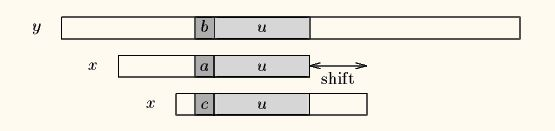
\includegraphics[width=0.7\textwidth]{gss1}
  \caption{Good-suffix shift, $u$ vuelve a aparecer en $x$ precedido por un carácter $c \neq a$}
	\label{gss1}
\end{figure}

Si no existe ese tipo de segmento, el movimiento consistirá en alinear el mayor sufijo $v$ de $y[j+i+1 \ \  ... \ \  j+m-1]$ con un prefijo coincidente de $x$ (ver figura \ref{gss2}).\\

\begin{figure}[H]
  \centering
    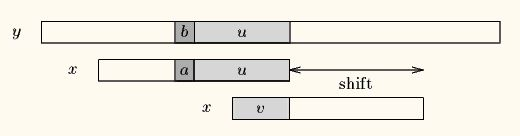
\includegraphics[width=0.7\textwidth]{gss2}
  \caption{Good-suffix shift, un sufijo de $u$ reaparece al principo de $x$}
	\label{gss2}
\end{figure}

El \textit{bad-character shift} consiste en alinear el carácter $y[i+j]$ con su aparición más a la derecha en $x[1 \ \  ... \ \  m-2]$ (ver figura \ref{bcs1}).\\

\begin{figure}[H]
  \centering
    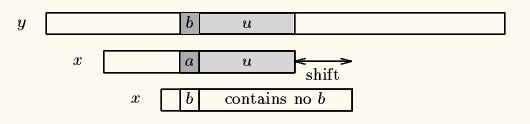
\includegraphics[width=0.7\textwidth]{bcs1}
  \caption{Bad-character shift, $b$ aparece en $x$}
	\label{bcs1}
\end{figure}

Si $y[i+j]$ no aparece en $x$, no habrá alineación posible de $x$ con $y[i+j]$, por lo que alinearemos $x[0]$ con $y[i+j+1]$(ver figura \ref{bcs2}).\\

\begin{figure}[H]
  \centering
    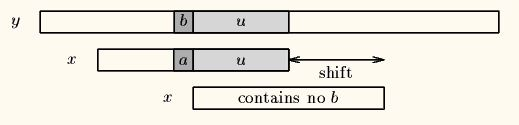
\includegraphics[width=0.7\textwidth]{bcs2}
  \caption{Bad-character shift, $b$ no aparece en $x$}
	\label{bcs2}
\end{figure}

Es interesante darse cuenta de que el \textit{bad-character shift} puede ser negativo, por lo tanto, el algoritmo elegirá el máximo valor arrojado por el \textit{good-suffix shift} y el \textit{bad-character shift} a la hora de hacer avanzar $x$ respecto a $y$.


%%%%%%%%%%Ejemplo%%%%%%%%%%
\subsection{Ejemplo del algoritmo de Boyer-Moore}
A continuación, se mostrará gráficamente el funcionamiento del algoritmo para un ejemplo concreto buscando un patrón en un texto en inglés. En cada paso, marcaremos con negrita el carácter en el que el algoritmo centra su atención.\\

\begin{align*} 
&x:     & &AT-THA\textbf{T}\\
&y: ... & &WHICH-\textbf{F}INALLY-HALTS.--AT-THAT-POINT ...\\
\end{align*}

Como `F' no aparece en $x$, usamos un \textit{bad-character-shift} (ver figura \ref{bcs2}) y desplazamos $x$:\\

\begin{align*} 
&x:     &        &AT-THA\ \textbf{T}\\
&y: ... & WHICH-F&INA\ LL\ Y\ \textbf{-}HALTS.--AT-THAT-POINT \ ...\\
\end{align*}

Ahora usamos otro \textit{bad-character-shift} (ver figura \ref{bcs1}) y desplazamos $x$ para alinear el espacio (-) de $y$ con el primer espacio (desde la derecha) de $x$:\\

\begin{align*} 
&x:     &        		 AT&-THA\textbf{T}\\
&y: ... & WHICH-FINALLY&-HAL\textbf{T}S.--AT-THAT-POINT ...\\
\end{align*}

Observamos que los caracteres visitados coinciden, por lo que movemos nuestra atención un carácter hacia la izquierda:\\

\begin{align*} 
&x:     &        		 AT&-TH\textbf{A}T\\
&y: ... & WHICH-FINALLY&-HA\textbf{L}TS.--AT-THAT-POINT ...\\
\end{align*}

Hacemos un \textit{bad-character-shift} (ver figura \ref{bcs2}) y, como `L' no aparece en $x$, avanzamos $m$ posiciones:\\

\begin{align*} 
&x:     &        					 &AT-THA\textbf{T}\\
&y: ... & WHICH-FINALLY-HAL&TS.\ \ --A\textbf{T}-THAT-POINT ...\\
\end{align*}

Ahora vemos que son los dos últimos caracteres de $x$ los que coinciden con $y$, por lo que movemos nuestra atención $2$ caracteres a la izquierda:\\

\begin{align*} 
&x:     &        					 &AT-T\textbf{H}AT\\
&y: ... & WHICH-FINALLY-HAL&TS.\ \ -\textbf{-}AT-THAT-POINT ...\\
\end{align*}

Finalmente, usamos un \textit{good-suffix-shift} (ver figura \ref{gss2}) de forma que encontramos una aparición de $x$ en $y$:\\

\begin{align*} 
&x:     &        				     	  &AT-THA\textbf{T}\\
&y: ... & WHICH-FINALLY-HALTS.--&AT-THA\textbf{T}-POINT ...\\
\end{align*}

Hemos de notar que solo hemos referenciado $y$ 14 veces, de las cuales 7 han sido para realizar la última comparación. Las otras 7 nos han permitido pasar los primeros 22 caracteres de $y$.


\section{El algoritmo}
A continuación concretaremos el algoritmo usando la notación de la sección \ref{sec:dnf}. Para optimizar la implementación del algoritmo, se realiza una fase de preprocesamiento en la que calculamos el valor que devolvería un \textit{bad-character-shift} y un \textit{good-suffix-shift} en cualquier situación. Para ello se construyen  dos tablas que concretaremos a continuación:\\

\subsection{Tabla del buen sufijo (GST)}
La primera será denominada la tabla del buen sufijo (GST). Para cada $i$ menor a $m$, construiremos el patrón consistente en los últimos $i$ caracteres de $x$ precedido por un carácter no coincidente con $x$. Es decir, construimos el patrón $c + x[m-1-i \ \ ...\ \ m-1]$ donde $c \neq x[m-2 -i]$ y $+$ representa la concatenación de caracteres. Ahora situaremos el patrón sobre $x$ y anotaremos el número mínimo de posiciones que hemos de mover el patrón a la izquierda para encontrar una coincidencia con $x$.\\

\begin{figure}[H]
  \centering
    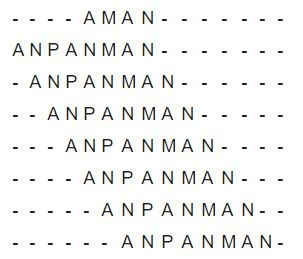
\includegraphics[width=0.45\textwidth]{gst}
  \caption{Tenemos $x[4] = N \neq A$, lo que nos obliga a desplazar $x$ seis caracteres a la izquierda.}
	\label{gst}
\end{figure}

Para la búsqueda de la cadena `ANPANMAN', la tabla sería la siguiente (`\sout{N}MAN' denotará a una cadena compuesta por un carácter diferente de `N' más los carácteres `MAN'): 

\begin{table}[H]
\begin{tabular}{|l|l|l|l|}
\hline
\rowcolor[HTML]{EFEFEF} 
\textbf{i} & \textbf{Patrón} & \textbf{Desp} & \textbf{Explicación}                                                                                                                                                           \\ \hline
0          & \sout{N}               & 1             & \begin{tabular}[c]{@{}l@{}}El penúltimo carácter de $x$ es diferente a `N',\\ con lo que basta desplazar una posición.\end{tabular}                                            \\ \hline
1          & \sout{A}N              & 8             & \begin{tabular}[c]{@{}l@{}}AN no es cadena en $x$ por lo que desplazaremos \\ $m = 8$.\end{tabular}                                                                             \\ \hline
2          & \sout{M}AN             & 3             & \begin{tabular}[c]{@{}l@{}}\sout{M}AN coincide con AN\textbf{PAN}MAN, por lo que \\ desplazamos 3 posiciones.\end{tabular}                                                                     \\ \hline
3          & \sout{N}MAN            & 6             & \begin{tabular}[c]{@{}l@{}}\sout{N}MAN no es subcadena de \textbf{ANPA}NMAN, pero el\\ final de \sout{N}MAN coincide con el inicio de $x$\\ (\sout{NM}\textbf{AN}PANMAN) por lo que desplazamos 6 posiciones.\end{tabular} \\ \hline
4          & \sout{A}NMAN           & 6             & Igual que $i=3$                                                                                                                                                                \\ \hline
5          & \sout{P}ANMAN          & 6             & Igual que $i=3$                                                                                                                                                                \\ \hline
6          & \sout{N}PANMAN         & 6             & Igual que $i=3$                                                                                                                                                                \\ \hline
7          & \sout{A}NPANMAN        & 6             & Igual que $i=3$                                                                                                                                                                \\ \hline
\end{tabular}
\end{table}

El algoritmo originalmente publicado por Boyer y Moore (ver \cite{articulo1}) usa una tabla más simple en la que no se requiere una no-coincidencia para el carácter de más a la izquierda. Sin embargo, esto no es suficiente para conseguir que el algoritmo funcione el tiempo lineal en el peor caso.

\subsection{Tabla del mal carácter (BCT)}
Para calcular esta tabla recorreremos $x$ de derecha a izquierda, empezando por el penúltimo carácter y pasando por todos. Si el carácter en el que nos encontramos no está aún en la tabla, lo añadimos con un desplazamiento asociado igual a su distancia hasta el último carácter. Es decir, si estamos en el carácter $x[i]$, y este aún no figura en la tabla, su desplazamiento asociado será $m - 1 - i$. A los caracteres que no figuren en $x$ se les asignará $m$. Para la cadena `ANPANMAN', la tabla quedaría de esta manera (por claridad, las entradas están ordenadas por orden de inserción): \\ 
 
\begin{table}[H]
\begin{tabular}{|l|l|}
\hline
\rowcolor[HTML]{EFEFEF} 
\textbf{Carácter}    & \textbf{Desplazamiento} \\ \hline
A                    & 1                       \\ \hline
M                    & 2                       \\ \hline
N                    & 3                       \\ \hline
P                    & 5                       \\ \hline
Caracteres restantes & 8                       \\ \hline
\end{tabular}
\end{table}


\subsection{Pseudocódigo}
A continuación se muestra mediante pseudocódigo el funcionamiento del algoritmo de Boyer-Moore (asumimos que tenemos las tablas GST y BCT ya rellenas): 

\begin{algorithm}[H]
\begin{algorithmic}[1]
\caption{Booyer-Moore Algorithm($x,y$)}
\STATE $j = 0$
\WHILE{$j \leq n - m$}
\IF{$x[0\ \ ...\ \ m-1] == y[j\ \ ...\ \ j+m-1]$}
\STATE Hay una coincidencia en $j$, la tratamos como corresponda.
\STATE $j += GST[0]$
\ELSE
\STATE $i =$ Posición en $x$ del primer carácter, contando desde la derecha, en el que difieran $x$ e $y$ ($x[i] \neq y[j + i]$).
\STATE $j += max(GST[i], BCT[y[i + j]] - (m - 1 - i))$
\ENDIF
\ENDWHILE
\end{algorithmic}
\end{algorithm}

\section{Implementación}
Se muestra a continuación una implementación del algoritmo de Boyer-Moore en C++:
\lstinputlisting[language=C++]{BM.cpp}


\section{Evidencia empírica}
En el artículo original publicado por Boyer y Moore (ver \cite{articulo1}) 
se presentaban los resultados de un test de eficiencia del algoritmo. Se ha considerado pertinente mostrar esos resultados aquí para comprobar de forma empírica la eficiencia del algoritmo.\\

El test selecciona aleatoriamente subpatrones de una secuencia base de caracteres. Se seleccionaron 300 subpatrones para cada longitud de subpatrón entre 1 y 14. Después se utilizaba el algoritmo de Boyer-Moore para buscar coincidencias, empezando desde una posición aleatoria de la primera mitad de la secuencia base. Se midió la eficiencia dividiendo el número de referencias a $y$ entre el número de caracteres de $y$ pasados durante el tiempo de ejecución del algoritmo. Esta medida es independiente de la implementación del algoritmo. Después se realizaría una media aritmética entre las 300 muestras de cada patrón.\\

Como la eficacia del algoritmo dependía de las propiedades estadísticas de $x$ e $y$, se realizó el test para tres textos distintos de 10000 caracteres cada uno. Uno era una secuencia aleatoria de 0's y 1's, otro era un texto en inglés obtenido de un manual online y el tercero era una secuencia aleatoria de caracteres de un diccionario de 100 caracteres. \\

\begin{figure}[H]
  \centering
    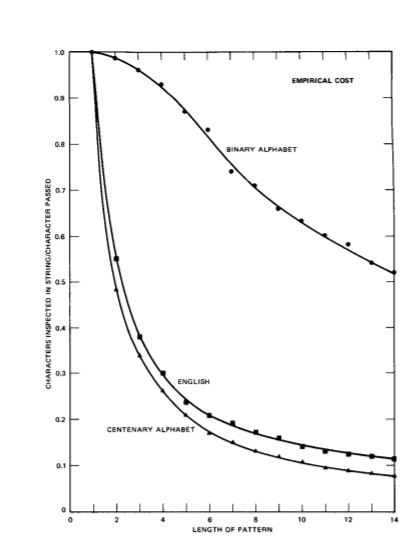
\includegraphics[width=0.45\textwidth]{performance}
	\label{performance}
\end{figure}

Los resultados del test muestran que la eficacia del algoritmo incrementa, para los tres textos, conforme aumenta la longitud del patrón buscado. Vemos que, a partir de los seis caracteres de longitud en los textos no binarios, el algoritmo solo referencia de media uno de cada cinco caracteres de $y$. Además, el ratio caracteres inspeccionados/caracteres pasados siempre es menor a uno (si $x$ consta de más de un carácter), es decir, el algoritmo mejora el coste lineal en estos casos.


\section{Rendimiento del algoritmo}
El problema del rendimiento del algoritmo no quedó zanjado en el artículo original publicado por Boyer y Moore (ver \cite{articulo1}). Ellos mostraron que el número de comparaciones no era mayor a $6n$, siendo $n$ el tamaño del texto donde el patrón es buscado. Más tarde, en 1980, se demostró que no era más de $4n$. Finalmente, en septiembre de 1991 Cole publicó un artículo (ver \cite{articulo2}) en el que mostraba que, en el caso peor, el algoritmo necesita aproximadamente $3n$ comparaciones  para encontrar todas las coincidencias, independientemente de si hay alguna o no. \\

Las demostraciones de estos resultados son largas y tediosas, por lo que se ha decidido no incluirlas aquí. Sin embargo, los artículos originales están referenciados al final del texto para que el lector pueda indagar más por su cuenta si así lo desea.

\section{Variantes}
A pesar de la eficiencia del algoritmo de Boyer-Moore, hay situaciones en las que es preferible utilizar variantes de este, ya sea para mejorar el rendimiento o para simplificar el código. A continuación se mostrarán dos de estas variantes:\\

\begin{itemize}
	\item \textbf{Algoritmo de Boyer-Moore Turbo}: Esta variante toma una cantidad adicional constante de espacio para completar una búsqueda en $2n$ comparaciones, mejorando el $3n$ del algoritmo normal.
	\item \textbf{Algoritmo de Boter-Moore-Horspool}: Es una simplificación del algoritmo que omite la GST. Con esta simplificación se requieren, en el caso peor, $nm$ comparaciones.
\end{itemize}


%%%%%%%%%%%%%%%%%%%%%%%%%%%%%%%%%%%%%%%%%%%%%%%%%%%%%%%%



\begin{thebibliography}{x}
\bibitem{articulo1} 
Boyer, R.S. y Moore, J.S. (1977). A Fast String Searching Algorithm. \textit{Communications of the ACM,20}(10), 762-772.

\bibitem{articulo2} 
Cole, R. (1991). Tight bounds on the complexity of the Boyer-Moore algorithm. \textit{Proceedings of the 2nd Annual ACM-SIAM Symposium on Discrete Algorithms}. 224-233.

\bibitem{wiki} 
Algoritmo de búsqueda de cadenas Boyer-Moore. Recuperado de: \url{https://es.wikipedia.org/wiki/Algoritmo_de_búsqueda_de_cadenas_Boyer-Moore#Rendimiento_del_algoritmo_de_búsqueda_de_cadenas_Boyer-Moore}

\bibitem{dibus}
Boyer-Moore algorithm. Recuperado de: \url{http://www-igm.univ-mlv.fr/~lecroq/string/node14.html}


\end{thebibliography}
\end{document}
